\section{Evaluation and critical appraisal}
\label{s:evaluation}

\subsection{Sensors energy measurements}

\begin{figure}[H]
\centering
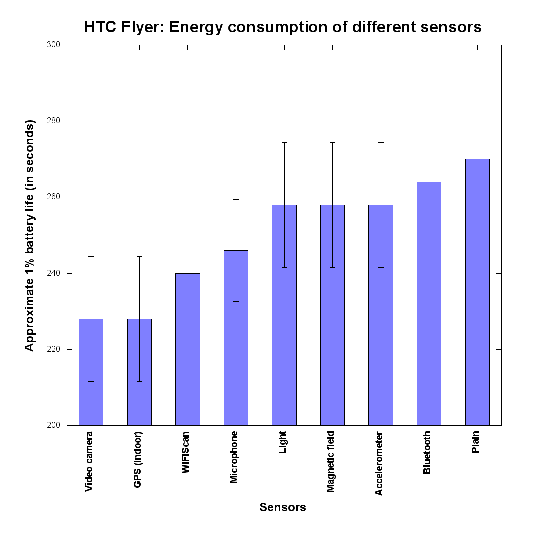
\includegraphics[width=0.49\textwidth, scale=0.6]{plots/htc_flyer}
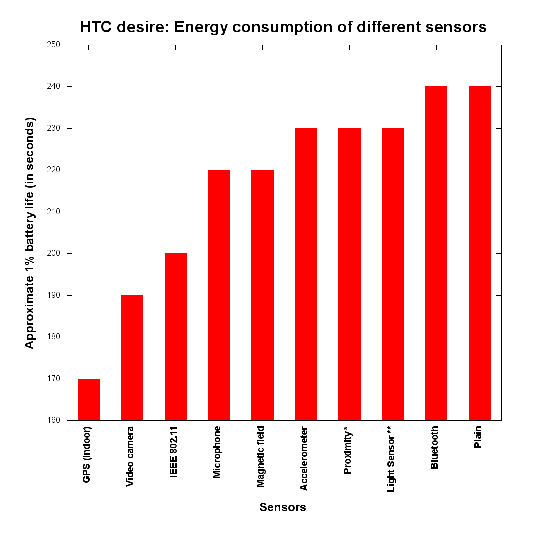
\includegraphics[width=0.49\textwidth, scale=0.6]{plots/htc_desire}
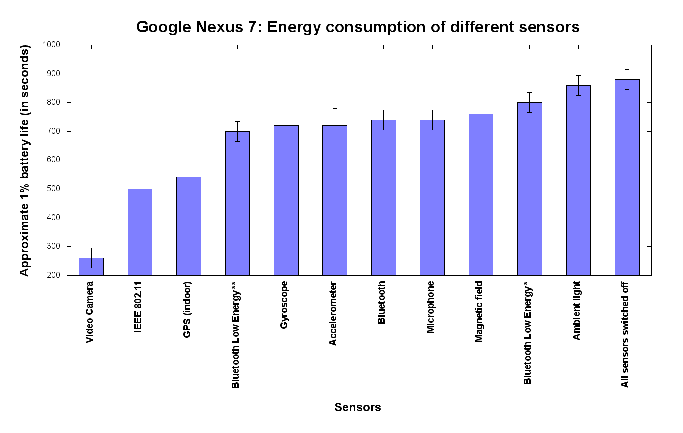
\includegraphics[width=\textwidth, scale=0.9]{plots/google_nexus_7}
\caption{\label{p:all_results} The complete results of energy measurements for all devices. The comparison of energy efficiency of different sensors is intuitive and overlaps with other research. }
\end{figure}


Those results are intuitive and overlap with other research.
	XXX all diagrams together
	plain run is the most energy-efficient
	physical sensors are relatively cheap
	microphone is a bit more expensive 
	wifi is even more expensive
	camera and gps have the highest energy demands
	XXX reference to some over research on it
	

The API issue: Bluetooth vs Bluetooth LE\\
	new functionality-> prints a lot of logs -> not energy-efficient\\
	XXX diagram: bluetooth vs bluetooth le 
	
\plot{bluetooth_le_api}
				
"the order" differs among devices\\
	gives the reason for online measurement\\
	disallows the usage of power models\\
		(need to look further into how they are built)\\
		related to fragmentation problem?!\\
	XXX diagrams: sensors in them same order -> different stairs
	
\begin{figure}[H]
\centering
\includegraphics[width=0.3\textwidth, scale=0.6]{plots/google_nexus_7_shared}
\includegraphics[width=0.3\textwidth, scale=0.6]{plots/htc_flyer_shared}
\includegraphics[width=0.3\textwidth, scale=0.6]{plots/htc_desire_shared}
\caption{\label{p:shared_sensors_results} Energy efficiency of shared sensors across different devices. The order of energy efficiency differs depending on a device. }
\end{figure}

physical sensors are relative cheap group of sensors \\
	this gives reason to leverage physical sensors for "expensive" sensors replacement
		for example versus GPS:
			XXX diagram acceleromter vs GPS
	however the difference is not so big, 
		(XXX the step equals to 1 thing)
		reasons: IPC, continuous sampling
			it gives better functionality; is more complex; uses more energy
		result: smart sampling of physical sensors needs to be leveraged
			-validates why people do duty-cycling, adaptive sampling
		this was shown before in XXX
	
\plot{acc_vs_loc}

Those results do not say anything on the cost when sensors are combined
		(crucial for providing some functionality out of physical sensors?)
		characteristics of cost? -> is it just CPU ?
			how WIFi and acceleromter vs wifi performs?
			how accelerometer and gyroscope vs acceleterometer performs?
				-intuition is that the result will not be much higher
			those questions are important for the idea behind  the library
				needs to be checked in practice separately.
		
		
\subsubsection{Localization}

The diagram of results across many devices for: camera, gps, wifi, microphone, bluetooth, bluetooth LE

\plot{all_locs}

XXX diagram all devices, sensors: GPS, Camera, Mic, WiFi, Bluetooth (order least to most)
WiFI may be cheaper than GPS
	reason why peoplpe prefer one over another				
				
microphone good results, people try to utilize it(research community)\\
				SurroundSense \cite{azizyan:surroundsense}\\
				however it's not always the cheapest\\
	
Bluetooth - is the cheapest in comparison to others
				exactly what industry does\\
				Bluetooth LE even accelerates those efforts
				References to beacons etc.\\
				(requires infrastructure)
				
Another on maybe computer vision, but:				\\
	Camera is the most expensive, and thus, not used yet for localization.\\
	
			
								
\subsection{Sensy}
\subsection{Conclusions}
Sensor energy measurements:
	-validation for the method
			as results overlap with other research
	-confirmation that Bluetooth LE API has problem with energy efficiency...
	-complete set of results across three different phones including all sensors
		-believed that first such measurement
	-different results among different devices-> reason why power model can't be used and there needs to be online measurements

other paragraph:
	Physical sensors:
		less expensive so can be leveraged for energy-efficient sensing
			-> validation for our library's design
		but provide more complex functionality, uses more energy
			require different strategies of using those "simple" sensors
				which gives a validation for movement detection in the library
		experiments does not say anything about combined values:
			how accelerometer+ wifi will be compared to acceleteremetor
				relevant for our energy-efficient library
	Results for localization: 
		-results explains why industry goes about it